\section{Results and Discussion}
\label{section:results}

Measurements from the EHT have yet to be collected. Therefore, we demonstrate the performance of our algorithm on synthetic examples. Figure~\ref{fig:results} illustrates how our algorithm's image reconstruction improves with an increasing number of telescopes in the array. Recall that as the number of telescopes, $N$, increases, the number of independent constraints on the reconstructed image increases as $\frac{(N-1)(N-2)}{2}$.The first reconstructed image in this figure is constrained using the triple products from a seven telescope array - the same number of telescopes expected to comprise EHT.  Since we have made no explicit assumption about the kind of image we expect to see in our prior model, we are able to reconstruct more complex images, such as the photogphag with only a few measurements.

\begin{figure}[h!]
\centering

{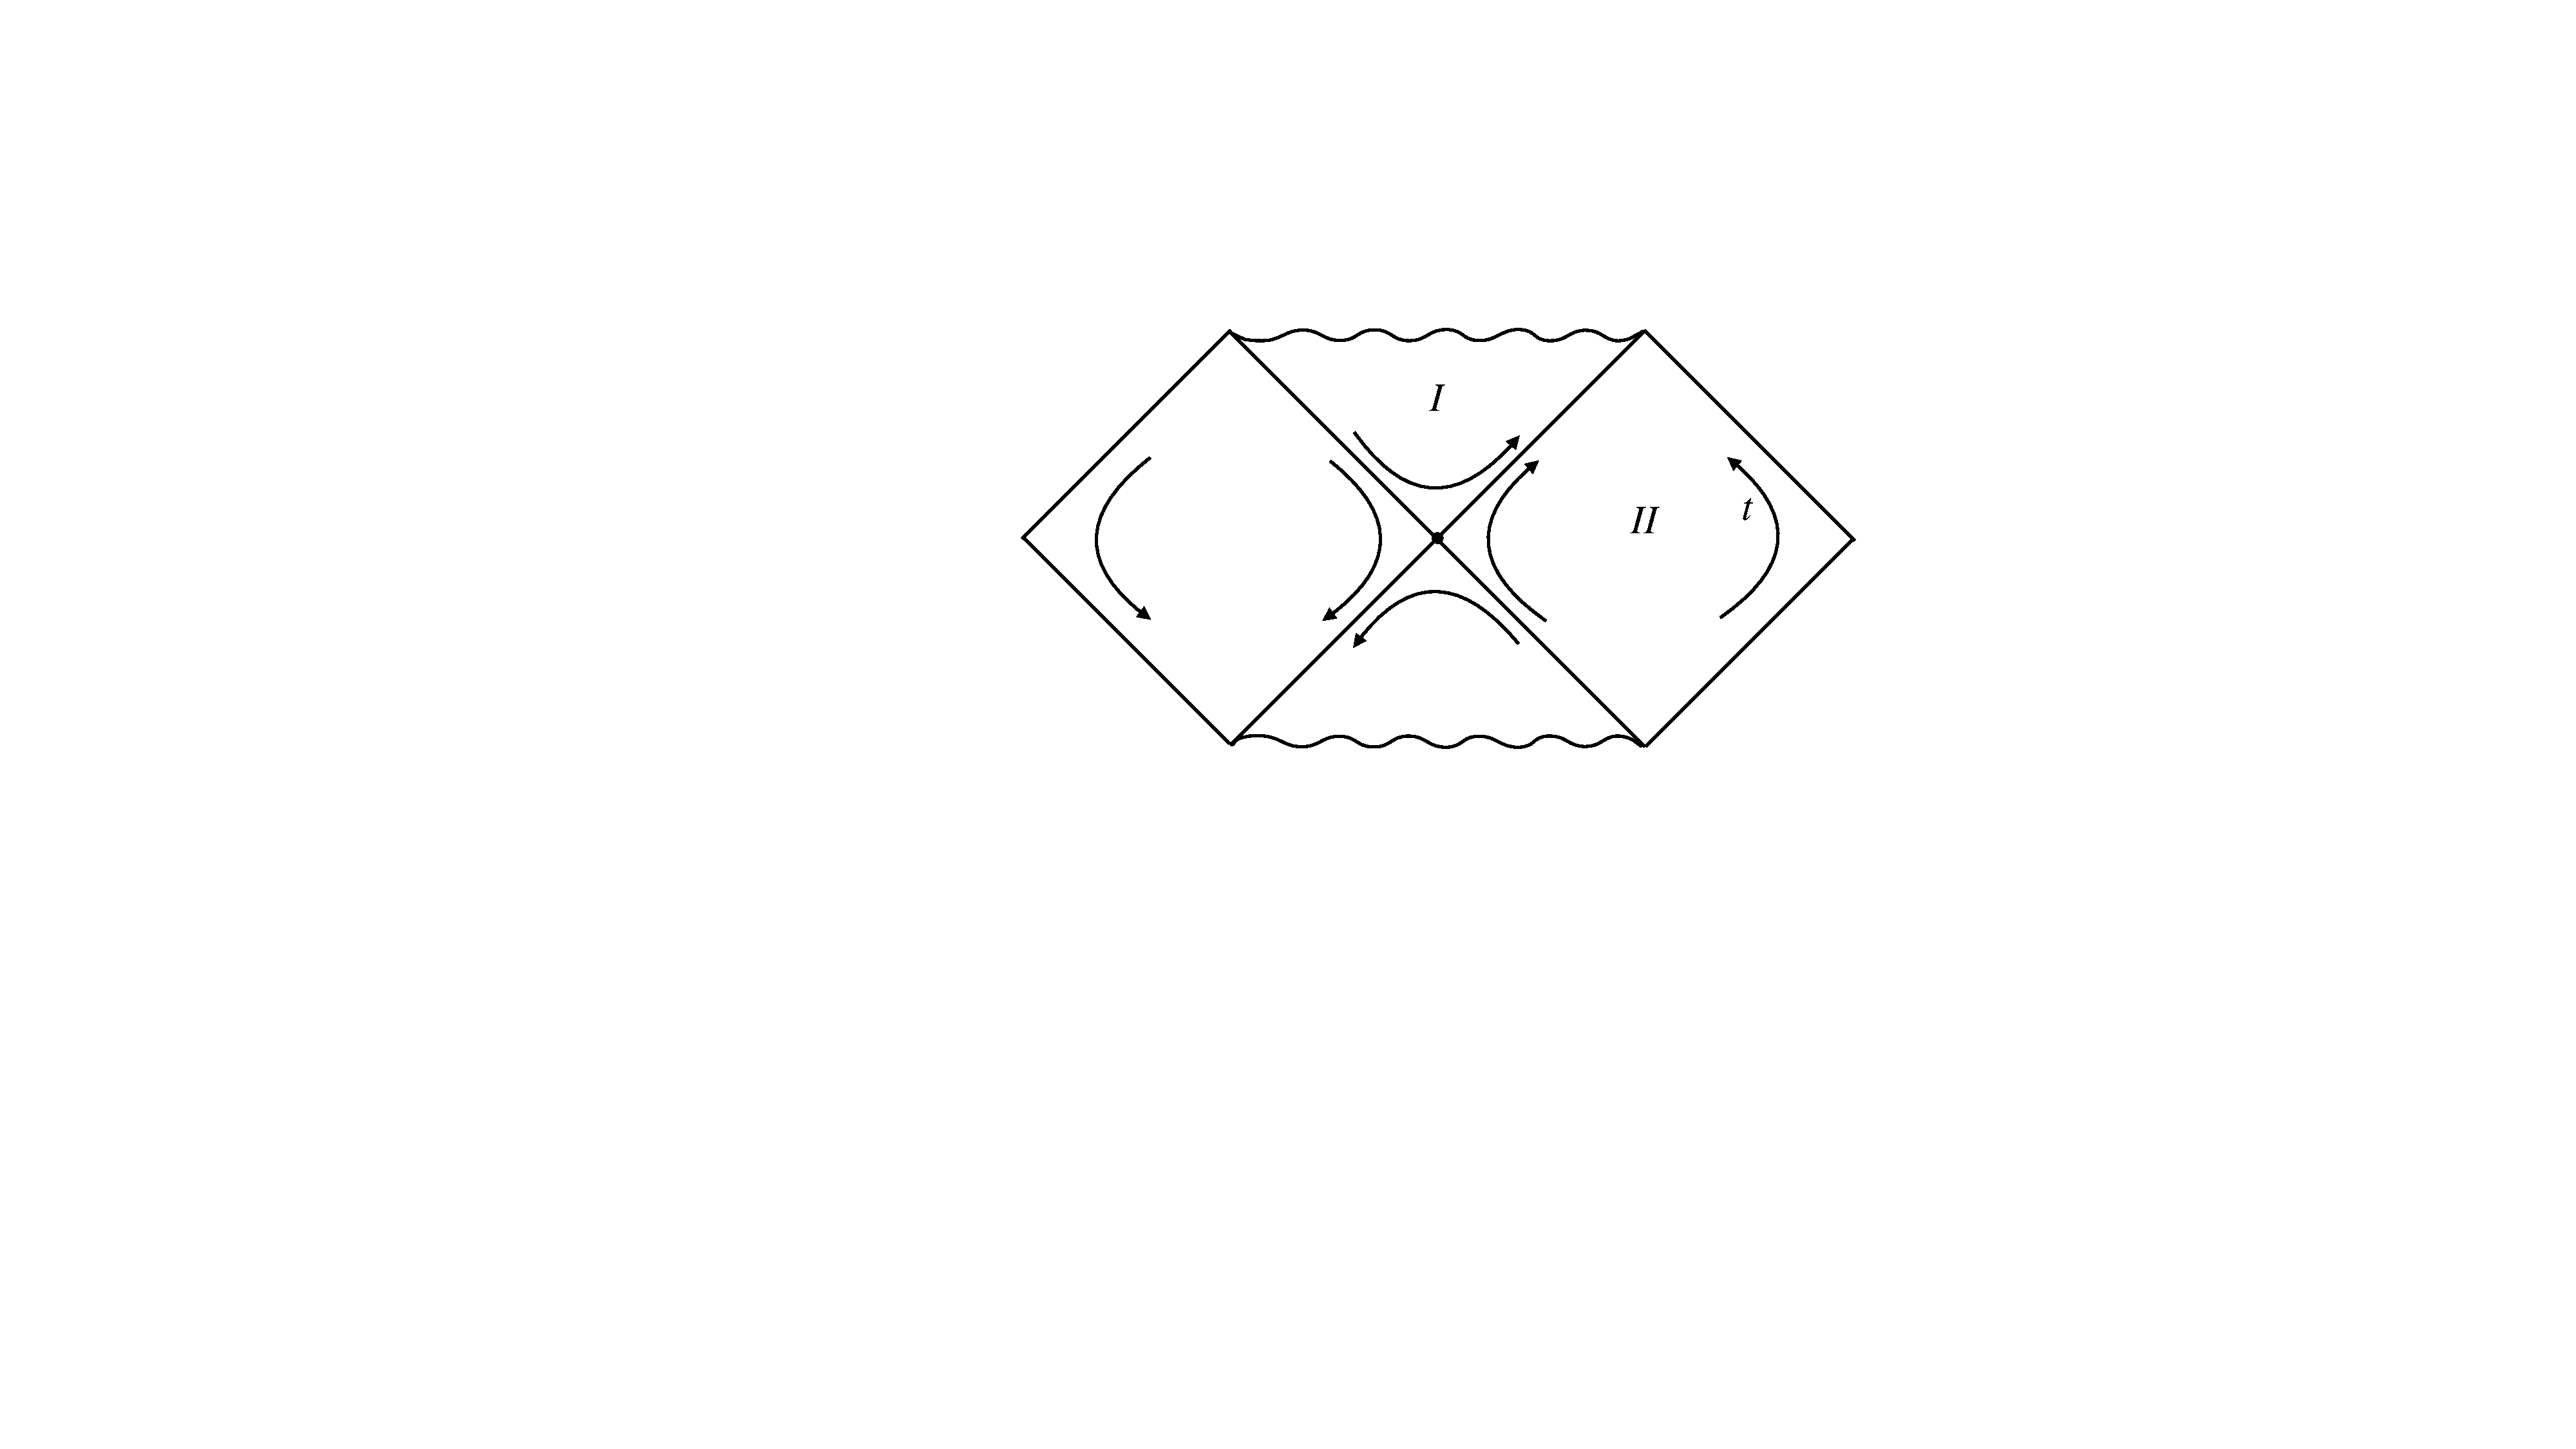
\includegraphics[width=.19\linewidth]
                   {images/eccvresults/bh.eps}}
{\includegraphics[width=.19\linewidth]
                   {images/eccvresults/bh7.eps}}
{\includegraphics[width=.19\linewidth]
                   {images/eccvresults/bh8.eps}}
{\includegraphics[width=.19\linewidth]
                   {images/eccvresults/bh9.eps}}  
{\includegraphics[width=.19\linewidth]
                   {images/eccvresults/bh10.eps}}  
                   
                   
{\includegraphics[width=.19\linewidth]
                   {images/eccvresults/lenna.eps}}
{\includegraphics[width=.19\linewidth]
                   {images/eccvresults/lenna7.eps}}
{\includegraphics[width=.19\linewidth]
                   {images/eccvresults/lenna8.eps}}
{\includegraphics[width=.19\linewidth]
                   {images/eccvresults/lenna9.eps}}  
{\includegraphics[width=.19\linewidth]
                   {images/eccvresults/lenna10.eps}}  
                   
                          \vspace{-.25in}
                      \[ \hspace{-.1in} \mbox{\footnotesize{Original Source}} \hspace{.2in} \mbox{\footnotesize{Increasing Number of Telescopes}} \xrightarrow{\hspace*{4cm}}  \]                                      
                        
                                      
                    \caption{{Increasing the number telescopes in a VLBI array improves the performance of our reconstruction algorithm. The original source in each row on the right (simulation of a black hole image and a test photograph) is shown reconstructed using from 7 to 10 different telescopes. In a 7 telescope array there are only 15 independent measurements of frequency information are available for reconstruction. In a 10 telescope the number of independent measurements increases to 36. Such a small number of constraints causes this inverse problem to be highly under-constrained. However, with the use of a generic image prior, we are able to start reconstructing images of even complex scenes. }}
 \label{fig:results}
\end{figure}


This example was generated from simulated elliptical trajectories along the $(u,v)$ plane. The sampled frequency measurements along these trajectories were then extracted from the ground truth image and corrupted by noise corresponding to a standard deviation of 20 degree error in the phase and a multiplicative error of standard deviation 5\% in the amplitude, as well as phase closure error due to atmospheric inhomogeneity.  We have assumed our source is non-varying, and thus have sampled all frequency components from the same underlying image. All images shown were reconstructed with $\Delta_\ell$ and $\Delta_m$ equal to 15\% of the largest frequency from the largest telescope array (10 telescopes). All trials were run using the same parameter set, and initialized with an $8 \times 8$ image containing random noise centered at the mean flux (average intensity).

\subsection{Interferometric Imaging Beauty Contest}

%In order to evaluate our algorithm against current st, we compare our reconstruction results to those produced by state of the art algorithms. 
The VLBI Imaging community has established a biennial ``beauty" contest where reconstruction algorithms compete to produce the best looking image using VLBI measurements. We qualitatively assess our algorithm's performance on the most recent competition, and compare our results to the results of the best performing algorithms. The full set of result images from competing algorithms can be seen at~\cite{baron20122012}. 

\begin{figure}[h!]
\centering

\subfigure[]{\includegraphics[height=.24\linewidth]
                   {images/eccvresults/alpuvcoverage.eps}}
\subfigure[]{\includegraphics[height=.24\linewidth]
                   {images/eccvresults/alpclosurephase.eps}}                                      
\subfigure[]{\includegraphics[height=.24\linewidth]
                   {images/eccvresults/betuvcoverage.eps}}
                   \subfigure[]{\includegraphics[height=.24\linewidth]
                   {images/eccvresults/betclosurephase.eps}}                
                                      
                    \caption{Data provided for reconstruction in the 2012 beauty contest challenge. The constrained components in the $(u,v)$ plane for Alp-Fak and Bet-Fak can be seen in (a) and (c) respectively. The complex values of the triple product are shown in red surrounded by a ellipse indicating one standard deviation of their error for Alp-Fak and Bet-Fak in (b) and (d) respectively. Measurements are taken at 8 different spectral channels (wavelengths). Therefore, due to the relationship $\beta/\lambda = (u,v)$, for every telescope pair, at every point in time, there are 8 measurements on the $(u,v)$ plane.   }
 \label{fig:data}
\end{figure}


In the 2012 beauty contest, two sets of VLBI measurements were provided for image reconstruction. We refer to these two data sets as Alp-Fak and Bet-Fak. VLBI measurements of Alp-Fak were produced from synthetic data (Figure~\ref{fig:beauty}a) using a realistic noise model and telescope array. This data contains measurements corresponding to a relatively dense sampling of the $(u,v)$ plane with a large covariance of noise around each measurement. The Bet-Fak measurements are actual measurements from a VLBI array of a Red Supergiant (Figure~\ref{fig:beauty}b). Although the variance of each measurement is smaller in this example than in Alp-Fak, there are much fewer measurements. The uv coverage and measurement noise can be seen in Figure~\ref{fig:data} for the two data sets. 

\begin{figure}[h!]
\centering

\subfigure[Alp-Fet Ground Truth]{\includegraphics[width=.35\linewidth]
                   {images/eccvresults/AlpOriginal.eps}}       
                   \qquad     
\subfigure[Bet-Fet Ground Truth]{\includegraphics[width=.35\linewidth]
                   {images/eccvresults/betOriginal.eps}}            

{\includegraphics[width=.23\linewidth]
                   {images/eccvresults/AlpSolution.eps}}                         
{\includegraphics[width=.23\linewidth]
                   {images/eccvresults/alp1.pdf}}        
{\includegraphics[width=.23\linewidth]
                   {images/eccvresults/alp2.pdf}}                  
{\includegraphics[width=.23\linewidth]
                   {images/eccvresults/alp3.pdf}}                           
                   
\subfigure[Our Algorithm]{\includegraphics[width=.23\linewidth]
                   {images/eccvresults/betresult.eps}}                         
\subfigure[1st Place]{\includegraphics[width=.23\linewidth]
                   {images/eccvresults/bet1.pdf}}        
\subfigure[2nd Place]{\includegraphics[width=.23\linewidth]
                   {images/eccvresults/bet2.pdf}}                  
\subfigure[3rd Place]{\includegraphics[width=.23\linewidth]
                   {images/eccvresults/bet3.pdf}}                        
                                      
                    \caption{{\bf Beauty Contest Comparison:} Results of our algorithm are comparable to these state of the art algorithms, despite the lack of a strong, restricted geometric image prior. The 2012 interferometry imaging beauty contest contains VLBI measurements from two sources - the synthetic image Alp-Fet (a) and real measurements of Bet-Fak (b). Researchers submitted reconstructions using the data. These reconstructions were then evaluated against the ground truth source images. We compare the reconstruction result of our algorithm using these measurements (a) against the top three winners of each challenge (d-f). Our reconstruction and the top reconstructions from the beauty contest for Alp-Fak and Bet-Fak are shown in the second and third row of this figure respectively.  All previous methods shown have used a disk prior model in reconstructing an image of Bet-Fak. However, our reconstruction was are able to reconstruct a disk image without explicitly including a disk model in our optimization.}
 \label{fig:beauty}
\end{figure}

Figure~\ref{fig:beauty}c shows the results of our algorithm and several state-of-the-art baseline algorithms on these two datasets. While our method's performance is qualitatively similar to the baseline methods, our method achieves these results with no assumptions about the shape or structure of the original body or scene. In contrast, the other methods assume a lot of a-priori structure information about the reconstructed image. For instance, in all competing algorithms, a disk prior model was used for reconstruction of Bet-Fak. Although we did not explicitly include a disk prior in our model, our algorithm was able to reconstruct a similar disk shape. A less restrictive prior is desirable since it is capable of generalizing better to more complex scenes, such as may be necessary in black hole images. 
%A more thorough evaluation of our method with current algorithms can be found in the supplemental material. 

%The result of our algorithm on the Alp-Fak and Bet-Fak data can be seen in Figure~\ref{fig:beauty}c. Although some of the detail is lost in the reconstructions, our algorithm is still able to resolve many of the large structures. Qualitatively, our results are comparable to those of the winning algorithms for each image. However,  unlike the other methods, which assume a lot of a-priori structure about the reconstructed image, our method uses a generic image prior and assumes very little about the global structure of the scene. For instance, in all competing reconstruction algorithms, a limb-darkened disk was used as a prior model of Bet-Fak. This strong prior model greatly helps in producing an image of a sharp disk object. However, our model was able to reconstruct a similar disk shape without this strong prior information. A more thorough evaluation of our method with current algorithms can be found in the supplemental material. 


%\subsection{Gridding}

%As mentioned previously, before optimization, current state of the art algorithms pre-process the data in order to place the frequency components on the DFT grid associated with a desired size image. However, this can cause errors that are not accounted for in optimization. In Figure BLAH we show the effect of using gridded frequencies rather than the actual measurements in our algorithm. 

\section{Conclusion}


In this paper we have presented an algorithm for reconstructing an image using a very sparse number of frequency constraints. This problem arises in the context of imaging celestial bodies using radio telescopes. This problem has a lot in common with many problems in the computer vision world - such as blind deconvolution, deblurring, super resolution, and in painting. We feel that by bridging the gap between these two areas, much of the work that has gone into developing good statistical image models can significantly improve results in the astrophysics community. 
